\documentclass{article}%
\usepackage[T1]{fontenc}%
\usepackage[utf8]{inputenc}%
\usepackage{lmodern}%
\usepackage{textcomp}%
\usepackage{lastpage}%
\usepackage[head=40pt,margin=0.5in,bottom=0.6in]{geometry}%
\usepackage{graphicx}%
%
\title{\textbf{Provea: Decreto de Emergencia Económica consolida la represión}}%
\author{José Andrade Godoy | jandrade@el{-}nacional.com}%
\date{18/09/2018}%
%
\begin{document}%
\normalsize%
\maketitle%
\textbf{URL: }%
http://www.el{-}nacional.com/noticias/politica/provea{-}decreto{-}emergencia{-}economica{-}consolida{-}represion\_252151\newline%
%
\textbf{Periodico: }%
EN, %
ID: %
252151, %
Seccion: %
Política\newline%
%
\textbf{Palabras Claves: }%
Política, Gobierno\newline%
%
\textbf{Derecho: }%
15, %
Otros Derechos: %
CONTEXTO, %
Sub Derechos: %
15.1\newline%
%
\textbf{EP: }%
NO\newline%
\newline%
%
\textbf{\textit{La ONG aseguró que la norma publicada en Gaceta Oficial Extraordinaria 41478 otorga el control de las finanzas públicas al Estado}}%
\newline%
\newline%
%
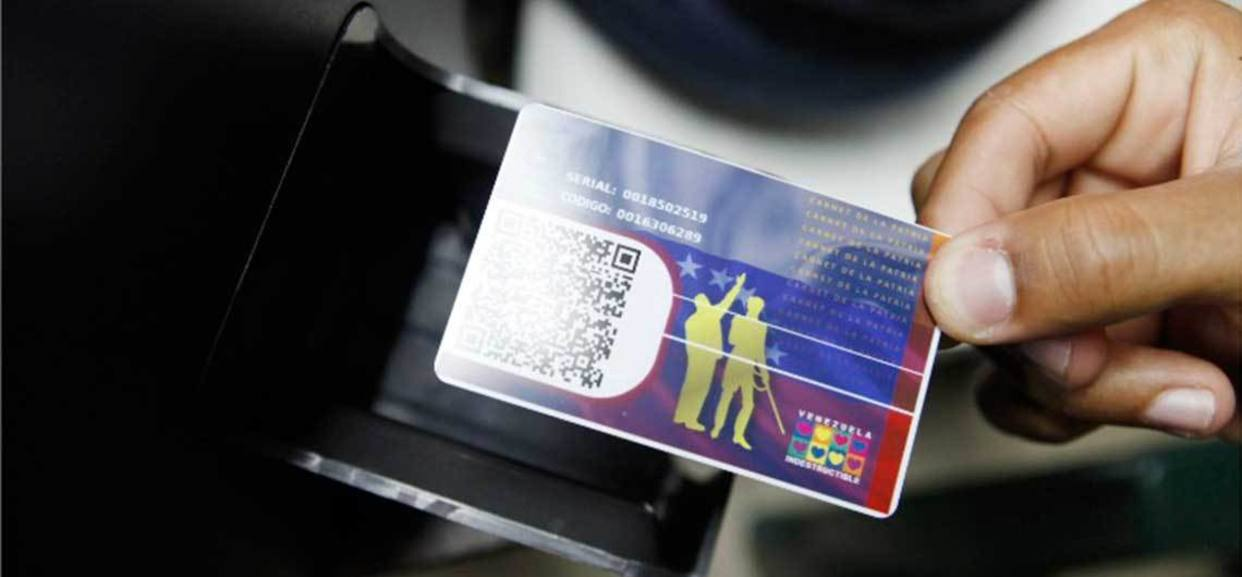
\includegraphics[width=300px]{249.jpg}%
\newline%
%
El decreto de Estado de Emergencia Económica dictado por Nicolás Maduro, en desconocimiento de las facultades de~la Asamblea Nacional, es un golpe más contra el Parlamento y constituye otro paso hacia la consolidación de mecanismos de control social, represión y cesión de la soberanía nacional a los “socios comerciales de la dictadura”, denunció el Programa Venezolano de Educación Acción en Derechos Humanos.%
\newline%
%
Provea señaló que~con el decreto 3.610 publicado en~Gaceta Oficial~Extraordinaria 41478~del 10 de septiembre, en el que se declara “Estado de Emergencia Económica en todo el territorio nacional”, el mandatario~viola el artículo 339 de~la Constitución“que establece que el decreto que declare el estado de excepción deberá ser declarado como constitucional por~la Asamblea Nacional~y el Tribunal Supremo de Justicia, ambos inclusive, cuestión de primer orden que no se plasmó en el contenido del referido decreto”.%
\newline%
%
Destacó que el artículo 11 del decreto otorga al mandatario la posibilidad de utilizar~sistemas de identificación y registro para controlar la aplicación subsidios y beneficios públicos,~y aseguró que la norma se implementó para justificar la imposición del carnet de la patria, “un mecanismo de control social y segregación política que ha sido promovido por la dictadura para limitar el acceso y disfrute de derechos por parte de la población”.%
\newline%
%
La ONG~advirtió que según los artículos 2 y 6 el gobierno “refuerza la respuesta represiva frente a las demandas ciudadanas y el descontento popular producto del hambre, el crecimiento de la pobreza y la indolencia gubernamental”. Agregó que pretenden amparar el uso de la fuerza por parte funcionarios policiales y militares para proteger los intereses del Estado por encima de los derechos de los ciudadanos.%
\newline%
%
“Los llamados planes especiales de seguridad pública ejecutados por Maduro han significado el aumento de los atropellos contra la población, como los ocurridos durante la ejecución del OLP, el aplastamiento de la protesta social en 2014 y 2017, el secuestro y la tortura de centenares de opositores políticos, y las más recientes e institucionalizadas masacres cometidas a diario por~la Fuerza~de Acciones Especiales de~la Policía Nacional~Bolivariana”, expresó la organización.%
\newline%
%
Provea rechazó la entrega de bienes del país a empresas multinacionales. “Un gobierno que se autocalifica como revolucionario, antiimperialista y defensor de la soberanía nacional, cede abiertamente la soberanía y los recursos del país a las transnacionales vinculadas a sus principales socios comerciales”.%
\newline%
%
El numeral 16 del artículo 2 del decreto 3.610 otorga al Ejecutivo la potestad de~“aprobar y suscribir contratos de interés público y sus enmiendas para la obtención de recursos financieros, asesorías técnicas o aprovechamiento de recursos estratégicos para el desarrollo económico del país, sin sometimiento a autorizaciones o aprobaciones de otros Poderes Públicos”.%
\newline%
%
Aseguró que con esta medida el presidente se atribuye competencias y “liquida la facultad exclusiva de~la Asamblea Nacional, contenida en el artículo 187 de~la Constitución”, además, afianza el manejo de las finanzas públicas y desconoce la labor de contraloría del Parlamento.%
\newline%
%
Recordó que no es la primera vez que el jefe del Estado dicta este tipo de medidas. “En 2016 se publicó, en~Gaceta Oficial~40855, el decreto número 2.248 con el cual se creó la~Zona de Desarrollo Estratégico Nacional Arco Minero del Orinoco. Mediante dicha norma Maduro entregó concesión para la explotación minera una extensión de 111.843 km2, que comprende 12,2\% del territorio nacional”.%
\newline%
%
\end{document}